\documentclass{article}

% Packages
\usepackage[english]{babel}
\usepackage[utf8]{inputenc}
\usepackage [autostyle]{csquotes}
\usepackage{graphicx}
\usepackage{tabularx}

\usepackage[style=authoryear]{biblatex} % Change "authoryear" to another style if preferred
\addbibresource{references.bib} % Link your .bib file

\newcommand{\chapsubhead}[1]{{\Large #1 \vspace{2ex}}}
\newcommand{\chaptype}[1]{{\Large \itshape (#1) \vspace{2ex}}}

\usepackage{graphicx}
\usepackage{pdfpages}
\usepackage{hyperref}
\usepackage{lipsum} % For generating dummy text, you can remove this package in your actual report

% Title, author, date
\title{Option Profit Calculator}
\author{Michael Martinez}
\date{\today} % Or specify a specific date

\begin{document}

\maketitle

\section{Background}
\indent In the age of digital stock brokerages and low-to-no commission trading, individuals have been empowered to make a wide range of investments across equities, derivatives, and cryptocurrencies safely and efficiently. Tools to help traders keep track of their own portfolio and monitor future investments are widespread, but can be locked behind paywalls (e.g. Snowball Analytics) or only offer a very specific service. The goal of this project is to outline a centralized application with a user-friendly interface as a trading and portfolio analytics tool specifically for traders that use Charles Schwab as their brokerage. The project is implemented entirely in Python so as to open up the project to customization by users in the future. 

\indent In this project, I aim to add three basic functionalities: 
\begin{enumerate}
    \item Interface to create an investment strategy based on different financial instruments.
    \item Given an investment strategy, the ability to simulate the possible profit/payoff that could occur in the future.
    \item A basic overview of a user's personal portfolio, with basic charting abilities.
\end{enumerate}

The final product will be an open-source GitHub repository that a user can easily clone into their own local machine, connect to their Charles Schwab brokerage account, and start the application on their machine to view their portfolio and chart investments. 

\indent For users that do not have access to Charles Schwab, a dummy dataset and portfolio will be made for demoing purposes. 

\indent This report will frequently use the term \enquote{option}, which is the name for a financial instrument that gives a buyer the option to buy or sell a stock or commodity. One stock or commodity can have hundreds of options contracts, even on the same day. These can be represented in an \enquote{options chain}, a tabular representation of all the options for one stock. Options have exploded in popularity recently because of their propensity for very high returns (or losses). They are also popular as a field of study in finance because of the mathematics that can be used to model their valuation. 

\section{Data Overview}

\indent All data is sourced using Schwab Developer (\cite{schwab_developer}), the official API for accessing market data through Charles Schwab's brokerage. To create a Schwab Developer account, you may follow these steps: 

\begin{itemize}
    \item Create a Schwab Developer account \href{https://developer.schwab.com/register}{here}. Note this account will be different than your Schwab brokerage/trading account, if you have one. 
    \item Once your account is created, navigate to the dashboard and click \enquote{Create App}
    \item Fill out the form to create an application. First, for "Select an API Product", add both \enquote{Accounts and Trading Production} and \enquote{Market Data Production} 
    \item Next, name the application (e.g. Derivatives Investment Tool)
    \item Add a short description (e.g. \enquote{Creating a tool to query market data to monitor my portfolio and chart investment strategies})
    \item Enter the callback URL: https://127.0.0.1 (this is the local host for your machine, and is used to get the necessary authentication tokens to access data)

\end{itemize}

\indent Once you have submitted the registration, Schwab Developer will approve your app for production. This usually takes 5-10 business days. Initially, the \enquote{Status} bar in the Dashboard will read \enquote{Approved - Pending}. Once it is approved, it will read \enquote{Ready For Use}. 

\indent Once the app is approved, you need to link your Schwab brokerage account with the Schwab Developer account. You can do this by following these steps: 
\begin{itemize}
    \item Clone the GitHub repository at this \href{https://github.com/mikemartinez13/option-profit-calculator}{link}.
    \item Follow the instructions in the README.md to set up the necessary packages. 
    \item Navigate to your Schwab Developer dashboard. Click \enquote{View Details} on your created app, find the \enquote{App Key} and \enquote{Secret Key}, and copy them. These will enable you to authenticate. 
    \item Follow the instructions in the README.md to set up the \enquote{.env} file. 
    \item Run ``authenticate.py''. This will take you to an authentication site, where you will use your Charles Schwab brokerage credentials (not Schwab Developer) to login. 
    \item After you've agreed to the terms and conditions, click the trading accounts you would like to link with Schwab Developer.

\end{itemize}

You may also refer to the README.md in \href{https://github.com/tylerebowers/Schwab-API-Python}{this GutHub repository} for an alternative guide to setting up Schwab Developer. 

\indent The raw format of the data provided by the Schwab Developer API is in JSON format. The API interface has multiple calls that allows the user to get quotes for stock, option data, personal account data, and more that can be accessed through the \enquote{requests} library in Python. An example of the output of a request is given in Figure~\ref{fig:Figure 1}.

\begin{figure}
    \begin{center}
    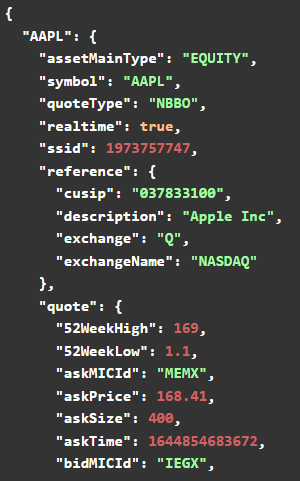
\includegraphics[scale=1]{example_quote.png}
    \caption{\label{fig:Figure 1}Raw output when requesting a quote for Apple stock.}
    \end{center}
\end{figure}



For more detailed information on data format, refer to the \href{https://developer.schwab.com/products/trader-api--individual/details/specifications/Market%20Data%20Production}{official Schwab Developer documentation} (Note you will need a Schwab Developer account to access this). 

\indent For the investment strategy builder, the code reorganizes the raw data into an options chain, which is displayed for the user to select the securities they would like to trade. An example of the options data is given in Figure~\ref{fig:Figure 2} (note the data has been split into two tables here for clarity): 


\begin{figure}[h]
    \centering

    \resizebox{\textwidth}{!}{%
    \begin{tabular}{lllllllll}
      & Contract Name         & Description             & Strike & Bid    & Ask    & Last   & Mark   & Delta \\
    0 & AAPL  241115C00005000 & AAPL 11/15/2024 5.00 C  & 5.0    & 221.35 & 222.85 & 0.0    & 222.1  & 1.0   \\
    1 & AAPL  241115C00010000 & AAPL 11/15/2024 10.00 C & 10.0   & 216.85 & 218.3  & 217.5  & 217.58 & 1.0   \\
    2 & AAPL  241115C00015000 & AAPL 11/15/2024 15.00 C & 15.0   & 211.85 & 213.3  & 212.95 & 212.58 & 1.0   \\
    3 & AAPL  241115C00020000 & AAPL 11/15/2024 20.00 C & 20.0   & 206.85 & 207.35 & 202.6  & 207.1  & 1.0   \\
    4 & AAPL  241115C00025000 & AAPL 11/15/2024 25.00 C & 25.0   & 201.8  & 202.85 & 202.1  & 202.33 & 1.0   \\
    5 & AAPL  241115C00030000 & AAPL 11/15/2024 30.00 C & 30.0   & 196.85 & 198.35 & 202.45 & 197.6  & 1.0   \\
    6 & AAPL  241115C00035000 & AAPL 11/15/2024 35.00 C & 35.0   & 191.85 & 192.85 & 0.0    & 192.35 & 1.0   \\
    7 & AAPL  241115C00040000 & AAPL 11/15/2024 40.00 C & 40.0   & 186.85 & 188.35 & 188.05 & 187.6  & 1.0   \\
    8 & AAPL  241115C00045000 & AAPL 11/15/2024 45.00 C & 45.0   & 180.0  & 183.25 & 0.0    & 181.63 & 1.0   \\
    9 & AAPL  241115C00050000 & AAPL 11/15/2024 50.00 C & 50.0   & 176.85 & 177.8  & 177.63 & 177.33 & 1.0  
    \end{tabular}%
    }
    \resizebox{\textwidth}{!}{%
    \begin{tabular}{lllllllll}
      & Gamma & Theta  & Vega & Rho   & ITM  & Intrinsic Value & Extrinsic Value & Days to Expiration \\
    0 & 0.0   & -0.019 & 0.0  & 0.001 & True & 221.96          & -221.96         & 6                  \\
    1 & 0.0   & -0.02  & 0.0  & 0.002 & True & 216.96          & 0.54            & 6                  \\
    2 & 0.0   & -0.021 & 0.0  & 0.003 & True & 211.96          & 0.99            & 6                  \\
    3 & 0.0   & -0.022 & 0.0  & 0.004 & True & 206.96          & -4.36           & 6                  \\
    4 & 0.0   & -0.022 & 0.0  & 0.005 & True & 201.96          & 0.14            & 6                  \\
    5 & 0.0   & -0.023 & 0.0  & 0.006 & True & 196.96          & 5.49            & 6                  \\
    6 & 0.0   & -0.023 & 0.0  & 0.007 & True & 191.96          & -191.96         & 6                  \\
    7 & 0.0   & -0.024 & 0.0  & 0.008 & True & 186.96          & 1.09            & 6                  \\
    8 & 0.0   & -0.025 & 0.0  & 0.009 & True & 181.96          & -181.96         & 6                  \\
    9 & 0.0   & -0.025 & 0.0  & 0.01  & True & 176.96          & 0.67            & 6                 
    \end{tabular}%
    }
    \caption{Example of an options chain.}
    \label{fig:Figure 2}
\end{figure}

Users here will be able to view key details about the different options they can choose for one expiration date. The \enquote{Contract Name} and \enquote{Description} columns give information about the official name of the option as well as key details about the underlying stock, expiration date, strike price, and type of option (\enquote{call} or \enquote{put}). The \enquote{Bid}, \enquote{Ask}, \enquote{Last}, and \enquote{Mark} columns give information about the current market price of the option. The \enquote{Delta}, \enquote{Gamma}. \enquote{Theta}, \enquote{Vega}, and \enquote{Rho} columns give technical details of how the value of the option changes with respect to different market factors, such as stock volatility or interest rates. The \enquote{ITM}, column stands for \enquote{In-the-Money}, which is a Boolean value that indicates whether the option can be exercised in the current moment or not. The \enquote{Intrinsic Value} column denotes the current value of an option when taking the difference between its strike price and the current stock price of the underlying asset. The \enquote{Extrinsic Value} represents the value of the option not made up by the Intrinsic Value, or in other words, the value of the option attributed to market factors such as volatility or specific excitement over a certain stock. Finally, the \enquote{Days to Expiration} column represents the time until the contract expires, when the value of the option becomes worthless.  

\section{Progress and Next Steps}

\indent Development of the project can be separated into the \enquote{backend}, the code that queries the API and calculates payoff for investment strategies, and the \enquote{frontend}, which designs the interface for the user to interact with. The backend originally used the Yahoo Finance API to query data, but it has been overhauled with the Schwab Developer API because of the query limits set on Yahoo Finance. Because the Schwab Developer API is complex and difficult to use directly, I used the \href{https://github.com/tylerebowers/Schwab-API-Python}{Schwabdev} Python library (\cite{schwabdev}) a wrapper to simplify my API calls. For data visualization, the \enquote{plots.py} file includes the code that allows users to create their own investment strategies using options, as well as code that visualizes the strategy's payoff over time using a heatmap. An example of an investment strategy payoff diagram is given in Figure~\ref{fig:Figure 3}, where profit is plotted against future stock price. For calculating option payoff, I used the \href{https://github.com/dbrojas/optlib/tree/master}{Optlib}  pricing library (\cite{optlib}). This makes up the bulk of the backend functionality, including data retrieval, pricing, and graphing. 

\begin{figure}
    \begin{center}
    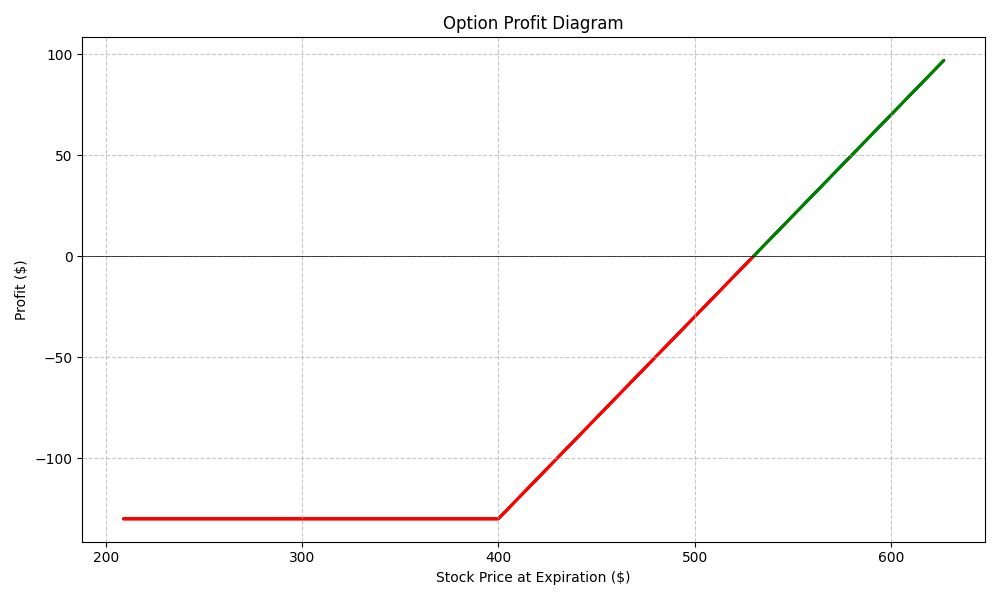
\includegraphics[width=\textwidth,height=\textheight,keepaspectratio]{long_call.png}
    \caption{\label{fig:Figure 3}Example of an investment strategy payoff graph.}
    \end{center}
\end{figure}


\indent My next major step is to design the frontend using the PyQt5 library. Since PyQt5 is a Python library, connecting to my backend Python code will be relatively simple compared to using React or other web-development languages. I plan to make at least three separate windows: one for users to select and view options, another for users to create strategies and view their payoffs, and one for users to view their personal portfolio account. If users do not have their personal trading account linked to Schwab, this last window will be disabled.  
After the frontend and the backend are integrated and linked together, I will create a README.md for the GitHub repository that will guide the user on how to set up Schwab Developer and how to use the application. The last step will be to modularize the code to perform specific tasks such as visualization, frontend, or pricing, and add documentation to enhance readability
for future users. 



\printbibliography

% \begin{thebibliography}{9} % The argument here is the widest label

% \bibitem{lamport1994latex}
%   Leslie Lamport,
%   \textit{LaTeX: A Document Preparation System},
%   Addison-Wesley, 2nd edition, 1994.

% \bibitem{knuth1984texbook}
%   Donald E. Knuth,
%   \textit{The \TeX{}book},
%   Addison-Wesley, 1984.

% \end{thebibliography}



\end{document} 
